% ===============================================================
%
% For tracking purposes - this is V2.0 - May 2012

\documentclass{sig-alternate}
%\graphicsextension{.ps,.eps}
\begin{document}
%
% --- Author Metadata here ---
\conferenceinfo{WOODSTOCK}{'97 El Paso, Texas USA}
%\CopyrightYear{2007} % Allows default copyright year (20XX) to be over-ridden - IF NEED BE.
%\crdata{0-12345-67-8/90/01}  % Allows default copyright data (0-89791-88-6/97/05) to be over-ridden - IF NEED BE.
% --- End of Author Metadata ---

\title{APEX: Autonomous Plan Verification and Execution}
%\subtitle{[Extended Abstract]
%\titlenote{A full version of this paper is available as
%\textit{Author's Guide to Preparing ACM SIG Proceedings Using
%\LaTeX$2_\epsilon$\ and BibTeX} at
%\texttt{www.acm.org/eaddress.htm}}}
%
\numberofauthors{4} 
%
\author{
% The command \alignauthor (no curly braces needed) should
% precede each author name, affiliation/snail-mail address and
% e-mail address. Additionally, tag each line of
% affiliation/address with \affaddr, and tag the
% e-mail address with \email.
%
% 1st. author
\alignauthor
Ben Trovato\titlenote{Dr.~Trovato insisted his name be first.}\\
       \affaddr{Institute for Clarity in Documentation}\\
       \affaddr{1932 Wallamaloo Lane}\\
       \affaddr{Wallamaloo, New Zealand}\\
       \email{trovato@corporation.com}
% 2nd. author
\alignauthor
G.K.M. Tobin\titlenote{The secretary disavows
any knowledge of this author's actions.}\\
       \affaddr{Institute for Clarity in Documentation}\\
       \affaddr{P.O. Box 1212}\\
       \affaddr{Dublin, Ohio 43017-6221}\\
       \email{webmaster@marysville-ohio.com}
% 3rd. author
\alignauthor Lars Th{\o}rv{\"a}ld\titlenote{This author is the
one who did all the really hard work.}\\
       \affaddr{The Th{\o}rv{\"a}ld Group}\\
       \affaddr{1 Th{\o}rv{\"a}ld Circle}\\
       \affaddr{Hekla, Iceland}\\
       \email{larst@affiliation.org}
\and  % use '\and' if you need 'another row' of author names
% 4th. author
\alignauthor Lawrence P. Leipuner\\
       \affaddr{Brookhaven Laboratories}\\
       \affaddr{Brookhaven National Lab}\\
       \affaddr{P.O. Box 5000}\\
       \email{lleipuner@researchlabs.org}
}
\date{\today}
% Just remember to make sure that the TOTAL number of authors
% is the number that will appear on the first page PLUS the
% number that will appear in the \additionalauthors section.

\maketitle
\begin{abstract}
This paper 
\end{abstract}

% A category with the (minimum) three required fields
\category{H.4}{Information Systems Applications}{Miscellaneous}
%A category including the fourth, optional field follows...
\category{D.2.8}{Software Engineering}{Metrics}[complexity measures, performance measures]

\terms{Theory}

\keywords{ACM proceedings, \LaTeX, text tagging}

\section{Introduction}
\label{introduction}

{\it Autonomy from human intervention in the machines that surround us promises many benefits.}

{\it Because of these benefits, autonomous and semi-autonomous systems are now an accepted part of the economy and the household.}

{\it Autonomous vehicles are a particularly challenging class of autonomous systems.}

{\it On a typical trip, the autonomous vehicle must recognize, enter, complete and exit many scenarios in a safe and timely manner. Example scenarios include traffic lights, roundabouts, pedestrians, weather conditions, etc. 
It is not known, ahead of time, what the specific sequence of encountered scenarios will be.}

{\it The corresponding technical challenges can be broadly divided into two categories: operation in a highly unpredictable environment, and a task (navigation) that must be executed at many levels of abstraction.}

{\it The environment of the autonomous vehicle is unpredictable: will others obey the laws, what will traffic conditions be, etc? What is the vehicle's objective in the short run?}

{\it There is also a wide separation between the highest levels of plan execution ("go from A to B") and the lowest levels of plan execution ("accelerate steadily for the next 5 seconds"). How do we guarantee consistency between the commands at the different levels?}

{\it The safety of the car's passengers and of the people in its immediate environment is imperative at all times. 
	What does safety mean in a given scenario?
	In an emergency, how do we recognize what laws can be broken to preserve safety?}

\todo[inline]{Safety,comfort,performance}
%\footnote{Interesting legal question: if the car, by design, violates some law to avoid harming someone, how long before the manufacturer gets sued for purposefully breaking the law? Think about swerving too hard and "losing control of the vehicle" to avoid running over someone.}
%\footnote{Other notions of safety, such as passive safety where the autonomous system must not endanger others via \emph{inaction}, or extensions of the safety imperative to not damaging property (and not just people) are not covered here. We note nonetheless that guaranteeing that the active safety imperative is obeyed contributes to guaranteeing these other notions are also obeyed.}
%For people to feel comfortable interacting with potentially dangerous autonomous agents, like autonomous cars, it is imperative that they be confident that these systems are at least as safe as the human-operated systems they are replacing.
%In fact, for there to be an economic value behind the introduction of autonomous systems, they must, among other things, guarantee an increased level of safety relative to the current system. 
%Increased and more consistent efficiency and effectiveness at completing their tasks are other desiderata, which are outside the scope of this paper.
%We call this the `dorasical' environment, from the Greek $\delta \rho \acute{\alpha} \sigma \eta$ for action.


{\it Guaranteeing safety to a socially acceptable degree requires formal guarantees.}

{\it Today we have theories that deal with high-level planning in a discrete grid world: where the car should go given where everyone else is.}

{\it We also have discrete theories for verification of temporal logic properties of the closed-loop system modeled as a Kripke structure. Some of these theories are amenable to model checking.}

{\it Control theory provides analysis and design tools of low level controllers. Automatic analysis tools exist but are limited in scope.}

{\it Because of the large degree of unpredictability, compute- and memory-intensive low level methods can't be used alone (let alone manual methods). Yet because of the safety imperative, we can't rely on non-guaranteed abstractions.  In this paper, we demonstrate the need for using multiple formalisms in the verification of autonomous plans. We illustrate this with a case study of a typical lane change maneuver.}

\begin{exmp}[Lane change maneuver]
	
	Throughout this work we will take as a case study the following example. At various instances we will zoom in on on specific scenarios within the sequence of events. The case study shows a target vehicle driving on a two lane road network that includes a merge which introduces another vehicle into the path of the target vehicle. The target vehicle's planning system may autonomously decide to initiate a lane change manuever to get around the other vehicle. The scenario terminates with an intersection governed by a traffic light. This scenario contains two vehicle agents (with different plans, 1 traffic control (infrastructure agent), and 1 road network. 
	
	\todo[inline]{who's involved in this scenario; what is the goal of ego vehicle; what is the sfaety constraint; why model checking alone won't suffice.}
\end{exmp}

From a planning perspective we define the safety of the discrete controller of the target vehicle to be the satisfaction of the following safety and liveness properties:
\begin{enumerate}
	\item The target vehicle may not exceed the speed limit (safety).
	\item The target vehicle may not collide with any other vehicles (if they exist) on the road (safety).
	\item The target vehicle must stop at a red light (safety).
	\item The target vehicle must eventually complete the scenario (liveness).
It is clearly possible to specify these properties using LTL operators (always and eventually).
\end{enumerate}

%Work on autonomous navigation: DARPA urban challenge papers, controller synthesis papers.
%
%DSL: that paper by the french authors, others?
%
%Scenarios and agents: there has to be a tonne here...the papers referenced by Matt in the APEX preso
%
%Interaction between model checkers and other verif tools: CEGAR, matthias and CMU guy, spaceex.
%
%Other semi-formal verif: staliro, breach, apx bisimulations.

\subsection{Notation}
We denote the set of integers including 0 with $\Ne$. 
Given a subset $S$ of the reals, $S^* = S \setminus \{0\}$ and $S_+ = S \cap [0,\infty)$,
while $S_+^* = S \cap (0,\infty)$.
\section{The modeling of autonomous plans}
\label{framework}

\begin{itemize}
	\item Scenarios and agents (don't dwell too long on this, just need to mention that we are verifying one scenario in this paper, but we have a plan for how this fits with overall mission verification)
	
	\item HCHA: because we need a representation rich enough to express on it different types of properties, which apply to different components of the complex autonomous vehicle
	
	\item Specification languages: should be suited to the verification goal. Here, reachability and LTL
	
\end{itemize}

\subsection{Decomposing a mission into scenarios and agents}
\label{scenarios and agents}
To motivate our thinking about the problem of safe autonomous navigation, we consider the case of a trip between two designated points.
On such a trip, the autonomous car will face a number of situations, or \emph{scenarios}, which it must know how to recognize, enter, negotiate, and exit in a safe and timely manner.
For example, the car will encounter roundabouts, 
traffic lights and four-way intersections, 
on-ramps to highways, 
lane changes, 
pedestrians,  
and various traffic signals like speed limits, school zones, etc.
We therefore think of a driving mission as an \emph{ordered sequence of scenarios}.
The exact sequence that will be encountered is not known ahead of time. 
%For example, it is not known whether some road has a large pothole that must be avoided.
Moreover, it is clear that some scenarios, like traffic lights, will be encountered more than once, albeit with minor site-specific differences. 
The key observation however is that the diversity of scenarios is, to a first order of approximation, finite. 
That is, there is a recognizable, finite set of scenario \emph{types} that is sufficient to describe most autonomous navigation missions.
The remaining variability among scenarios can be parametrized: e.g., the number of cars at a roundabout, or the current speed limit.

To formally define a scenario, we first outline its elements.
First, within each scenario, we can recognize a recurring set of entities: 
the autonomous vehicle whose operation we seek to verify (a.k.a. the \emph{ego} vehicle), the other vehicles on the road, pedestrians, traffic signage, and the road network itself. 
We will refer to these as \emph{agents}: an agent is an entity that functions continuously and autonomously in the environment, and whose presence can be sensed by other agents. 
\todo[inline]{main literature for agents}
Formally, we recognize the following set of four agent \emph{types}, whose semantics are given in the next section.
\[\agentTypeSet = \{\texttt{vehicle, pedestrian, road, trafficSignage}\}\]
Each agent type can have many (parametrized) instances, e.g. $\texttt{trafficSignage}$ can have instances speedLimit(70mph), speedLimit(25mph), HOVLane(3pm-6pm).
We denote the set of instances of agents in $\agentTypeSet$ by $I(\agentTypeSet)$.
Clearly, $I(\agentTypeSet)$ is infinite.
When we just speak of an agent, we mean an agent instance.

Formally, we define a scenario instance as follows. 
The elements of a scenario will be formally defined in the following sections.
\begin{defn}[Scenario instance]
	A scenario instance is a tuple $(\agentInstanceSet,\behavior, \lawSet, \Phi, Init, \exitConditions)$ where
\begin{itemize}
	\item $A$ is a collection of agent \emph{instances} from the set $I(\agentTypeSet)$.
	The set $\agentInstanceSet$ always includes the ego vehicle, i.e., the system whose behavior we want to verify.
	%
	\item $\behavior = \{\behavior_a \sut a \in \agentInstanceSet \setminus \{egoVehicle\}\}$ is a bounded-time behavior description for each of the other agent instances.
	Describing the behavior $\behavior_a$ of an agent instance requires us to formally describe an agent. 
	We do so in Section \ref{HCHA}.
	What assumptions we make on the behavior of other vehicles is captured in $\behavior$.
	%
	\item $\lawSet = \{l_0,\ldots,l_p\}$ is a finite set of $p \in \Ne$ traffic laws. 
	A law $l_i$ is a temporal logic formula indicating how the law constrains the behavior of the ego vehicle, but not the other agents. 
	I.e. it is a specification on the ego vehicle that must be satisfied. 
	% 
	\item $\Phi$ is a set of goals that must be met by the ego vehicle while in this scenario. 
	Now $\Phi$ and $\lawSet$ may both be expressed as (temporal) logic specifications on the system's behavior and therefore may be grouped together as one set.
	However it helps to keep these two aspects of the scenario separate: 
	that laws are constraints on the vehicle's behavior, and scenario goals are objectives to be met.
	%
	\item $Init$ is an initialization of the scenario, which defines a valid initial set of states for the agents when the scenario starts. $Init$ is formally defined in the next section.
	% 
	\item $\exitConditions$ is a set of condition describing how and when the scenario ends.
	The conditions are described as temporal logic formulae with atomic propositions on the states of the agents in the scenario.
	The formulae are required to be satisfiable by finite prefixes.
	That is, for any formula $\formula \in \exitConditions$, if there exists a trace $\sttraj$ of the system that satisfies $\formula$, then there exists a finite prefix of $\sttraj$ that satisfies $\formula$.
\end{itemize}
Let $\Sc = \{s_0,s_1,\ldots,s_{N-1}\}$ be a set of scenario instances. 
Then \textbf{a mission} $M$ is a finite string on $\Sc$, $M \in \Sc^*$.
\end{defn}

\todo[inline]{mission as an automaton?}

The logic in which a law $l_i$ or exit condition $\formula_i$ is expressed will depend on the formalism used to model the scenario's agents. 
We will have more to say about this in the following sections.

Because a mission is a sequence of scenarios, if we can verify the safety of the autonomous system's behavior in each scenario,
and compose the scenarios in a safe manner, 
then we have verified that the mission is safe.
In the rest of this paper we formalize the correct composition of scenarios and illustrate it with a case study in Section \ref{caseStudy}.
Note that in this paper, we do not study how to \emph{generate} missions for verification. 
Rather we assume that we are given mission to be verified. 
The problem of mission generation and verification coverage will be the subject of future research.

\begin{prob}[Correct composition of scenarios]
	
	\end{prob}


\begin{exmp}[Lane change continued]
	The mission can be decomposed into the following scenarios:
	$M = $ DriveStraight, ChangeLane, PassOnTheLeft, StopAtFourWayIntersection.
	Each of these scenarios contains two instances $v_{ego}$ and $v_2$ of the \texttt{vehicle} agent type, one \texttt{road} agent instance, no \texttt{pedestrian}s and one \texttt{trafficSignage} agent.
	The behavior $\behavior_{v_2}$ is given by a sequence of reach sets as detailed in Section \ref{otherAgents};
	briefly, $\behavior_{v_2}$ gives the area occupied by $v_2$ at any moment in time.
	An example applicable law, expressed in discrete time LTL, is $l \defeq \always(position_{ego} = a \implies X position_{ego} \geq a)$, to indicate that backing up is not allowed.
	Note that LTL is not ideally suited for this requirement since we need one formula per speed threshold $a$. A more concise logic (e.g., TPTL \cite{alur94_really}) would allow us to directly say $l \defeq \always(position_{ego}(t+1) \geq position_{ego}(t))$, while still being reasonably computationally tractable.
		
	There are two exit conditions for the DriveStraight scenario: either the ego vehicle reaches the end of the current road segment (i.e. , it reaches the intersection). 
	Or, it gets too close to the leading vehicle $v_2$, in which case it must exit and scenario ChangeLane begins.
	The $Init$ set for ChangeLane is the union of two sets $Init_1$ and $Init_2$.
	$Init_1$ is the set of 2D positions on the road where $v_ego$ is behind $v_2$ and within some distance $d_{min}$ of $v_2$.
	$Init_2$ is the set of 2D positions of $v_{ego}$ that are some distance $d_{turn}$-close to the intersection.
	I.e., we consider the lane change to be provoked by excessive proximity to the leading vehicle $v_2$, or by proximity to the intersection.	
\end{exmp}

It should be noted that the initialization of a scenario may have a mission-dependent part, like $Init_2$ in the example.
This highlights the need to do verification \emph{in the context of the mission}, as the context provides information on what needs to be verified.
	
%	E.g an instance of scenario $s_0$ (Roundabout) might have the agents 
%	\begin{eqnarray*}
%		\agentInstanceSet = \{&egoVehicle, otherVehicle1, rndAbt(3), \\ 
%		& speedLimit(25mph)\} \subset I(\agentTypeSet)
%	\end{eqnarray*}
%	where $egoVehicle$ and $otherVehicle1$ are instances of type $\texttt{vehicle}$, 
%	$rndAbout(n)$ is an instance of $\texttt{road}$ indicating a round-about with $n$ entry points (which are also exit points),
%	and $speedLimit(Vmph)$ is an intance of $\texttt{trafficSignage}$ indicating a speed limit sign that reads $V$ mph.
%	Another scenario instance has the agents
%	\begin{eqnarray*}
%		\agentInstanceSet = \{&EgoVehicle, OtherVehicle1, rndAbt(2), \\ 
%		& speedLimit(35mph)\} \subset I(\agentTypeSet)
%	\end{eqnarray*}
%	

\subsection{Hierarchical communicating hybrid \\automata}
\label{HCHA}
Because autonomous systems are physical systems controlled by software, hybrid automata (HA) are a suitable formalism for modeling them.
Because the complexity of autonomous systems is significant, they are typically designed at multiple levels of abstraction, 
with different teams handling the design at different levels.
E.g. the mapping team might design the algorithm for finding the waypoints along a shortest route from start to end.
For this design, knowledge about, say, the powertrain control of the car is immaterial and abstracted away.
Indeed, details about the road itself are abstracted away as well.
Instead, it is represented as a directed graph.

The resulting system's description is given at multiple levels of abstraction (or multiple levels of detail). 
To model this situation, we adopt \emph{hierarchical} HA: each mode of the HA is itself an HA, down to some level.

Finally because these HHA, each representing an agent, are sensed by other agents in the scenario, we must model this sensing. 
We do so via the inputs to each HHA: given agent instance $a$, every other agent is associated with an input port on $a$.
When that other agent is within sensing distance of $a$, that input port is occupied by that agent's sensed information.


\todo[inline]{Refer to Charon}


\subsection{What is safety?}
\label{safety}

For people to feel comfortable interacting with potentially dangerous autonomous agents, like autonomous cars, it is imperative that they be confident that these systems are at least as safe as the human-operated systems they are replacing.
In fact, for there to be an economic value behind the introduction of autonomous systems, they must, among other things, guarantee an increased level of safety relative to the current system. 
Increased and more consistent efficiency and effectiveness at completing their tasks are other desiderata, which are outside the scope of this paper.

In this section, we formalize the safety imperative: 
that is, what it means for an autonomous system to be safe, in the context of autonomous vehicles.
\todo[inline]{lit review on safety}
The general (active) safety imperative is that the autonomous car must not take actions that directly endanger the car's passengers (including the driver) or people in the environment that is susceptible to its actions.
We call this the `dorasical' environment, from the Greek $\delta \rho \acute{\alpha} \sigma \eta$ for action.
\footnote{Other notions of safety, such as passive safety where the autonomous system must not endanger others via \emph{inaction}, or extensions of the safety imperative to not damaging property (and not just people) are not covered here. We note nonetheless that guaranteeing that the active safety imperative is obeyed contributes to guaranteeing these other notions are also obeyed.}

For an autonomous vehicle, this safety requirement means not colliding with other agents in the environment (cars, pedestrians, and traffic signage), or entering unsafe regions of the environment, like opposing traffic lanes or obstacles.
This holds regardless of the scenario type the ego vehicle is engaged in. 
But specializing this imperative to a given scenario type allows us to break it down into more specific requirements which, when formally expressed, can facilitate the model checking task.
Intuitively, by specifying certain ways in which safety can be violated, we guide the model checker towards finding those ways, in effect constraining the search space.
\todo[inline]{cite XOR (formalize => prove)? (in that order)}
These scenario-appropriate properties are then expressed in a formal logic like Linear Temporal Logic (LTL) \cite{Pnueli77sfcs} or Metric Temporal Logic (MTL) \cite{Koymans90}, and formally verified on the formal model of the scenario.
To avoid confusing common terminology, we will call these \emph{safety-inducing properties}, because when we write them as logic formulae they don't take the form of what is usually referred to as a safety formula. 
That is, they are not in the form $\always (x \notin \text{Unsafe set})$.
But once they are satisfied, they guarantee, by construction, that the safety imperative is satisfied in this scenario.
\todo[inline]{Future: Can we take the absolute safety mandates and automatically specialize them to scenarios? I.e. given the set of state trajectories of the car, automatically derive, from the scenario, some constraints that constrain the search for the subset of trajectories that end in harming someone in that particular scenario?}
\todo[inline]{safety algebara?}
 % scenarios, agents and hierarchical communicating HA
\section{Design entry and the tool bus}
\label{designEntryAndToolBus}

\subsection{The tool bus}
\label{tool bus}
One of our goals in APEX is to formally verify the safety of the autonomous system's operation in all scenario types.
As we saw in Section \ref{safety}, the imperative to be safe is expressed by different logic properties in the different scenarios types.
To verify these properties, we must first decide on the appropriate formalism(s) in whic to express them (e.g. LTL, CTL, or MTL?) 
and the corresponding formalism for describing the autonomous system under verificaiton.
Secondly, we must decide on which tool to run to verify the property.
In general, we may expect that different properties, and different levels of abstraction at which they are verified, will require (or be better verified) using different formalisms and tools. 
For example, verifying a property of the continuous-time dynamics may be done using {\staliro}~\cite{AnnapureddyLFS11tacas},
whereas verifying a property of the discrete mission planner may be best done using UPPAAL \cite{BehrmannDLHPYH06qest}.
This motivates the creation of a translator from our detailed HCHA representation of the scenario instance to the different formalisms that are deemed useful. 
For example: timed automata, weighted timed automata, Ordinary Differential Equation (ODEs), impulsive systems,...etc.
See Fig.~\ref{fig:toolbus}.

\begin{figure}[tb]
	\centering
		\includegraphics{figures/fly.eps}
	\label{fig:toolbus}
	\caption{The APEX tool bus.}
\end{figure}

The representation of a scenario and its agents in some Intermediate Representation (IR) allows the translation into many other formalisms.
The key requirement is that the IR must be at least as detailed as any target formalism.
Formally, we say that a model $\Mc_1$ (in formalism $F_1$, e.g. HCHA) is at least as detailed as model $\Mc_2$ (in formalism $F_2$, e.g. timed automata) if the behavior of $\Mc_2$ contains the behavior of $\Mc_1$: 
\[\behavior_{\Mc_1} \subset \behavior_{\Mc_2}\]
This is the familiar notion of behavior inclusion, and it is one more reason for choosing HCHA as the IR:
the most detailed analysis that can be made on the autonomous system is at the level of the continuous dynamics.
These are captured in the HCHA. 
Other aspects are also captured in the HCHA, as explained in Section \ref{HCHA}.
These details can be abstracted when translating the HCHA to a timed automaton to perform verification using UPPAAL.
On the other hand, had we chosen timed automata as our IR, we would not have been able to recover the true dynamics from the timed automaton's differential inclusions. This would preclude us from performing accurate reachability computations for example.

\todo[inline]{a word on jhow to transfer verif results back to HCHA}

APEX includes a tool bus: once a combination of tools is decided on for a particular verification task, the IR is translated to the formats of these tools and transmitted to them.

\subsection{Simulation model}
\label{simulation model}
Control engineers, who will be one of the main group of users of APEX, are mostly used to \emph{simulating} their designs under certain initial conditions and inputs from the environment to determine correctness. 
Simulation is also a quick way to get a qualitiative idea of what the system does, and is used iteratively to improve the design.
It is therefore important for APEX to provide a translation from the IR to a simulation tool, in addition to the translation to formal tools. 
We chose to add the MathWorks' Simulink \copyright to the tool bus.
Simulink is well-known to most engineers and has the advantage of a Graphical User Interface which can be leveraged as a design entry tool (see Section \ref{dsl}).

Note that because the simulation model will not be subjected to formal verification, there is no need to establish behavioral inclusion between its behavior and the IR.


\subsection{Scenario authoring tool and Domain-Specific Language}
\label{dsl}
How are the scenarios created? DSL and scenario authoring tool.
\input{
\section{Introduction}
The \textit{proceedings} are the records of a conference.
ACM seeks to give these conference by-products a uniform,
high-quality appearance.  To do this, ACM has some rigid
requirements for the format of the proceedings documents: there
is a specified format (balanced  double columns), a specified
set of fonts (Arial or Helvetica and Times Roman) in
certain specified sizes (for instance, 9 point for body copy),
a specified live area (18 $\times$ 23.5 cm [7" $\times$ 9.25"]) centered on
the page, specified size of margins (1.9 cm [0.75"]) top, (2.54 cm [1"]) bottom
and (1.9 cm [.75"]) left and right; specified column width
(8.45 cm [3.33"]) and gutter size (.83 cm [.33"]).

The good news is, with only a handful of manual
settings\footnote{Two of these, the {\texttt{\char'134 numberofauthors}}
and {\texttt{\char'134 alignauthor}} commands, you have
already used; another, {\texttt{\char'134 balancecolumns}}, will
be used in your very last run of \LaTeX\ to ensure
balanced column heights on the last page.}, the \LaTeX\ document
class file handles all of this for you.

The remainder of this document is concerned with showing, in
the context of an ``actual'' document, the \LaTeX\ commands
specifically available for denoting the structure of a
proceedings paper, rather than with giving rigorous descriptions
or explanations of such commands.

\section{The {\secit Body} of The Paper}
Typically, the body of a paper is organized
into a hierarchical structure, with numbered or unnumbered
headings for sections, subsections, sub-subsections, and even
smaller sections.  The command \texttt{{\char'134}section} that
precedes this paragraph is part of such a
hierarchy.\footnote{This is the second footnote.  It
starts a series of three footnotes that add nothing
informational, but just give an idea of how footnotes work
and look. It is a wordy one, just so you see
how a longish one plays out.} \LaTeX\ handles the numbering
and placement of these headings for you, when you use
the appropriate heading commands around the titles
of the headings.  If you want a sub-subsection or
smaller part to be unnumbered in your output, simply append an
asterisk to the command name.  Examples of both
numbered and unnumbered headings will appear throughout the
balance of this sample document.

Because the entire article is contained in
the \textbf{document} environment, you can indicate the
start of a new paragraph with a blank line in your
input file; that is why this sentence forms a separate paragraph.

\subsection{Type Changes and {\subsecit Special} Characters}
We have already seen several typeface changes in this sample.  You
can indicate italicized words or phrases in your text with
the command \texttt{{\char'134}textit}; emboldening with the
command \texttt{{\char'134}textbf}
and typewriter-style (for instance, for computer code) with
\texttt{{\char'134}texttt}.  But remember, you do not
have to indicate typestyle changes when such changes are
part of the \textit{structural} elements of your
article; for instance, the heading of this subsection will
be in a sans serif\footnote{A third footnote, here.
Let's make this a rather short one to
see how it looks.} typeface, but that is handled by the
document class file. Take care with the use
of\footnote{A fourth, and last, footnote.}
the curly braces in typeface changes; they mark
the beginning and end of
the text that is to be in the different typeface.

You can use whatever symbols, accented characters, or
non-English characters you need anywhere in your document;
you can find a complete list of what is
available in the \textit{\LaTeX\
User's Guide}\cite{Lamport:LaTeX}.

\subsection{Math Equations}
You may want to display math equations in three distinct styles:
inline, numbered or non-numbered display.  Each of
the three are discussed in the next sections.

\subsubsection{Inline (In-text) Equations}
A formula that appears in the running text is called an
inline or in-text formula.  It is produced by the
\textbf{math} environment, which can be
invoked with the usual \texttt{{\char'134}begin. . .{\char'134}end}
construction or with the short form \texttt{\$. . .\$}. You
can use any of the symbols and structures,
from $\alpha$ to $\omega$, available in
\LaTeX\cite{Lamport:LaTeX}; this section will simply show a
few examples of in-text equations in context. Notice how
this equation: \begin{math}\lim_{n\rightarrow \infty}x=0\end{math},
set here in in-line math style, looks slightly different when
set in display style.  (See next section).

\subsubsection{Display Equations}
A numbered display equation -- one set off by vertical space
from the text and centered horizontally -- is produced
by the \textbf{equation} environment. An unnumbered display
equation is produced by the \textbf{displaymath} environment.

Again, in either environment, you can use any of the symbols
and structures available in \LaTeX; this section will just
give a couple of examples of display equations in context.
First, consider the equation, shown as an inline equation above:
\begin{equation}\lim_{n\rightarrow \infty}x=0\end{equation}
Notice how it is formatted somewhat differently in
the \textbf{displaymath}
environment.  Now, we'll enter an unnumbered equation:
\begin{displaymath}\sum_{i=0}^{\infty} x + 1\end{displaymath}
and follow it with another numbered equation:
\begin{equation}\sum_{i=0}^{\infty}x_i=\int_{0}^{\pi+2} f\end{equation}
just to demonstrate \LaTeX's able handling of numbering.

\subsection{Citations}
Citations to articles \cite{bowman:reasoning,
clark:pct, braams:babel, herlihy:methodology},
conference proceedings \cite{clark:pct} or
books \cite{salas:calculus, Lamport:LaTeX} listed
in the Bibliography section of your
article will occur throughout the text of your article.
You should use BibTeX to automatically produce this bibliography;
you simply need to insert one of several citation commands with
a key of the item cited in the proper location in
the \texttt{.tex} file \cite{Lamport:LaTeX}.
The key is a short reference you invent to uniquely
identify each work; in this sample document, the key is
the first author's surname and a
word from the title.  This identifying key is included
with each item in the \texttt{.bib} file for your article.

The details of the construction of the \texttt{.bib} file
are beyond the scope of this sample document, but more
information can be found in the \textit{Author's Guide},
and exhaustive details in the \textit{\LaTeX\ User's
Guide}\cite{Lamport:LaTeX}.

This article shows only the plainest form
of the citation command, using \texttt{{\char'134}cite}.
This is what is stipulated in the SIGS style specifications.
No other citation format is endorsed or supported.

\subsection{Tables}
Because tables cannot be split across pages, the best
placement for them is typically the top of the page
nearest their initial cite.  To
ensure this proper ``floating'' placement of tables, use the
environment \textbf{table} to enclose the table's contents and
the table caption.  The contents of the table itself must go
in the \textbf{tabular} environment, to
be aligned properly in rows and columns, with the desired
horizontal and vertical rules.  Again, detailed instructions
on \textbf{tabular} material
is found in the \textit{\LaTeX\ User's Guide}.

Immediately following this sentence is the point at which
Table 1 is included in the input file; compare the
placement of the table here with the table in the printed
dvi output of this document.

\begin{table}
\centering
\caption{Frequency of Special Characters}
\begin{tabular}{|c|c|l|} \hline
Non-English or Math&Frequency&Comments\\ \hline
\O & 1 in 1,000& For Swedish names\\ \hline
$\pi$ & 1 in 5& Common in math\\ \hline
\$ & 4 in 5 & Used in business\\ \hline
$\Psi^2_1$ & 1 in 40,000& Unexplained usage\\
\hline\end{tabular}
\end{table}

To set a wider table, which takes up the whole width of
the page's live area, use the environment
\textbf{table*} to enclose the table's contents and
the table caption.  As with a single-column table, this wide
table will ``float" to a location deemed more desirable.
Immediately following this sentence is the point at which
Table 2 is included in the input file; again, it is
instructive to compare the placement of the
table here with the table in the printed dvi
output of this document.


\begin{table*}
\centering
\caption{Some Typical Commands}
\begin{tabular}{|c|c|l|} \hline
Command&A Number&Comments\\ \hline
\texttt{{\char'134}alignauthor} & 100& Author alignment\\ \hline
\texttt{{\char'134}numberofauthors}& 200& Author enumeration\\ \hline
\texttt{{\char'134}table}& 300 & For tables\\ \hline
\texttt{{\char'134}table*}& 400& For wider tables\\ \hline\end{tabular}
\end{table*}
% end the environment with {table*}, NOTE not {table}!

\subsection{Figures}
Like tables, figures cannot be split across pages; the
best placement for them
is typically the top or the bottom of the page nearest
their initial cite.  To ensure this proper ``floating'' placement
of figures, use the environment
\textbf{figure} to enclose the figure and its caption.

This sample document contains examples of \textbf{.eps}
and \textbf{.ps} files to be displayable with \LaTeX.  More
details on each of these is found in the \textit{Author's Guide}.

\begin{figure}
\centering
\epsfig{file=fly.eps}
\caption{A sample black and white graphic (.eps format).}
\end{figure}

\begin{figure}
\centering
\epsfig{file=fly.eps, height=1in, width=1in}
\caption{A sample black and white graphic (.eps format)
that has been resized with the \texttt{epsfig} command.}
\end{figure}


As was the case with tables, you may want a figure
that spans two columns.  To do this, and still to
ensure proper ``floating'' placement of tables, use the environment
\textbf{figure*} to enclose the figure and its caption.
and don't forget to end the environment with
{figure*}, not {figure}!

\begin{figure*}
\centering
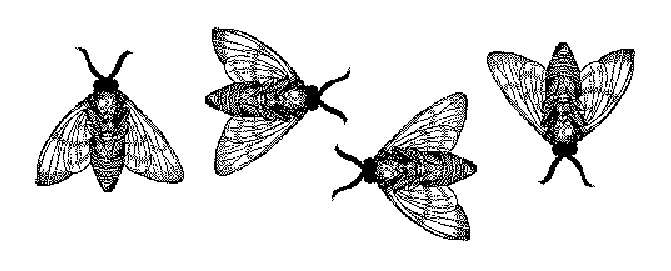
\epsfig{file=flies.eps}
\caption{A sample black and white graphic (.eps format)
that needs to span two columns of text.}
\end{figure*}

Note that either {\textbf{.ps}} or {\textbf{.eps}} formats are
used; use
the \texttt{{\char'134}epsfig} or \texttt{{\char'134}psfig}
commands as appropriate for the different file types.

\begin{figure}
\centering
\psfig{file=rosette.ps, height=1in, width=1in,}
\caption{A sample black and white graphic (.ps format) that has
been resized with the \texttt{psfig} command.}
\vskip -6pt
\end{figure}

\subsection{Theorem-like Constructs}
Other common constructs that may occur in your article are
the forms for logical constructs like theorems, axioms,
corollaries and proofs.  There are
two forms, one produced by the
command \texttt{{\char'134}newtheorem} and the
other by the command \texttt{{\char'134}newdef}; perhaps
the clearest and easiest way to distinguish them is
to compare the two in the output of this sample document:

This uses the \textbf{theorem} environment, created by
the\linebreak\texttt{{\char'134}newtheorem} command:
\newtheorem{theorem}{Theorem}
\begin{theorem}
Let $f$ be continuous on $[a,b]$.  If $G$ is
an antiderivative for $f$ on $[a,b]$, then
\begin{displaymath}\int^b_af(t)dt = G(b) - G(a).\end{displaymath}
\end{theorem}

The other uses the \textbf{definition} environment, created
by the \texttt{{\char'134}newdef} command:
\newdef{definition}{Definition}
\begin{definition}
If $z$ is irrational, then by $e^z$ we mean the
unique number which has
logarithm $z$: \begin{displaymath}{\log e^z = z}\end{displaymath}
\end{definition}

Two lists of constructs that use one of these
forms is given in the
\textit{Author's  Guidelines}.
 
There is one other similar construct environment, which is
already set up
for you; i.e. you must \textit{not} use
a \texttt{{\char'134}newdef} command to
create it: the \textbf{proof} environment.  Here
is a example of its use:
\begin{proof}
Suppose on the contrary there exists a real number $L$ such that
\begin{displaymath}
\lim_{x\rightarrow\infty} \frac{f(x)}{g(x)} = L.
\end{displaymath}
Then
\begin{displaymath}
l=\lim_{x\rightarrow c} f(x)
= \lim_{x\rightarrow c}
\left[ g{x} \cdot \frac{f(x)}{g(x)} \right ]
= \lim_{x\rightarrow c} g(x) \cdot \lim_{x\rightarrow c}
\frac{f(x)}{g(x)} = 0\cdot L = 0,
\end{displaymath}
which contradicts our assumption that $l\neq 0$.
\end{proof}

Complete rules about using these environments and using the
two different creation commands are in the
\textit{Author's Guide}; please consult it for more
detailed instructions.  If you need to use another construct,
not listed therein, which you want to have the same
formatting as the Theorem
or the Definition\cite{salas:calculus} shown above,
use the \texttt{{\char'134}newtheorem} or the
\texttt{{\char'134}newdef} command,
respectively, to create it.

\subsection*{A {\secit Caveat} for the \TeX\ Expert}
Because you have just been given permission to
use the \texttt{{\char'134}newdef} command to create a
new form, you might think you can
use \TeX's \texttt{{\char'134}def} to create a
new command: \textit{Please refrain from doing this!}
Remember that your \LaTeX\ source code is primarily intended
to create camera-ready copy, but may be converted
to other forms -- e.g. HTML. If you inadvertently omit
some or all of the \texttt{{\char'134}def}s recompilation will
be, to say the least, problematic.

\section{Conclusions}
This paragraph will end the body of this sample document.
Remember that you might still have Acknowledgments or
Appendices; brief samples of these
follow.  There is still the Bibliography to deal with; and
we will make a disclaimer about that here: with the exception
of the reference to the \LaTeX\ book, the citations in
this paper are to articles which have nothing to
do with the present subject and are used as
examples only.
%\end{document}  % This is where a 'short' article might terminate

%ACKNOWLEDGMENTS are optional
\section{Acknowledgments}
This section is optional; it is a location for you
to acknowledge grants, funding, editing assistance and
what have you.  In the present case, for example, the
authors would like to thank Gerald Murray of ACM for
his help in codifying this \textit{Author's Guide}
and the \textbf{.cls} and \textbf{.tex} files that it describes.

%
% The following two commands are all you need in the
% initial runs of your .tex file to
% produce the bibliography for the citations in your paper.
\bibliographystyle{abbrv}
\bibliography{sigproc}  % sigproc.bib is the name of the Bibliography in this case
% You must have a proper ".bib" file
%  and remember to run:
% latex bibtex latex latex
% to resolve all references
%
% ACM needs 'a single self-contained file'!
%
%APPENDICES are optional
%\balancecolumns
\appendix
%Appendix A
\section{Headings in Appendices}
The rules about hierarchical headings discussed above for
the body of the article are different in the appendices.
In the \textbf{appendix} environment, the command
\textbf{section} is used to
indicate the start of each Appendix, with alphabetic order
designation (i.e. the first is A, the second B, etc.) and
a title (if you include one).  So, if you need
hierarchical structure
\textit{within} an Appendix, start with \textbf{subsection} as the
highest level. Here is an outline of the body of this
document in Appendix-appropriate form:
\subsection{Introduction}
\subsection{The Body of the Paper}
\subsubsection{Type Changes and  Special Characters}
\subsubsection{Math Equations}
\paragraph{Inline (In-text) Equations}
\paragraph{Display Equations}
\subsubsection{Citations}
\subsubsection{Tables}
\subsubsection{Figures}
\subsubsection{Theorem-like Constructs}
\subsubsection*{A Caveat for the \TeX\ Expert}
\subsection{Conclusions}
\subsection{Acknowledgments}
\subsection{Additional Authors}
This section is inserted by \LaTeX; you do not insert it.
You just add the names and information in the
\texttt{{\char'134}additionalauthors} command at the start
of the document.
\subsection{References}
Generated by bibtex from your ~.bib file.  Run latex,
then bibtex, then latex twice (to resolve references)
to create the ~.bbl file.  Insert that ~.bbl file into
the .tex source file and comment out
the command \texttt{{\char'134}thebibliography}.
% This next section command marks the start of
% Appendix B, and does not continue the present hierarchy
\section{More Help for the Hardy}
The sig-alternate.cls file itself is chock-full of succinct
and helpful comments.  If you consider yourself a moderately
experienced to expert user of \LaTeX, you may find reading
it useful but please remember not to change it.
%\balancecolumns % GM June 2007
% That's all folks!
\end{document}
